\documentclass[aspectratio=169]{beamer}
%
% Choose how your presentation looks.
%
% For more themes, color themes and font themes, see:
% http://deic.uab.es/~iblanes/beamer_gallery/index_by_theme.html
%
\mode<presentation>
{
  \usetheme{default}      % or try Darmstadt, Madrid, Warsaw, ...
  \usecolortheme{default} % or try albatross, beaver, crane, ...
  \usefonttheme{default}  % or try serif, structurebold, ...
  \setbeamertemplate{navigation symbols}{}
  \setbeamertemplate{caption}[numbered]
} 

\usepackage[english]{babel}
\usepackage[export]{adjustbox}
 % \usepackage[utf8x]{inputenc}
\usepackage[style=authoryear]{biblatex}
\addbibresource{references.bib}
\usepackage{tikz}
\usepackage{xcolor}
\usepackage{relsize}
\usepackage[absolute,overlay]{textpos}
\graphicspath{{figures/}}
\DeclareMathOperator{\sign}{sign}

\usepackage{caption}
\captionsetup{font=scriptsize, labelfont=scriptsize}

\newcommand{\specialcell}[2][c]{%
  \begin{tabular}[#1]{@{}c@{}}#2\end{tabular}}

\title[Your Short Title]{When does vapor pressure deficit drive or reduce evapotranspiration?}
\author{Adam Massmann,  Pierre Gentine and Changjie Lin}
\institute{AGU Fall Meeting}
\date{December 14th, 2017}

\begin{document}

\begin{frame}
  \titlepage
\end{frame}


\section{Introduction}


\begin{frame}{Does VPD drive or reduce ET? - atmospheric demand perspective}
  \begin{columns}
    \begin{column}{0.7\textwidth}
      Increase in VPD (\textbf{increase in atmospheric demand}) drives  an \textbf{increase in ET}.
      \[VPD = (1-RH)\cdot e_s (T)\]
    \end{column}
    \begin{column}{0.3\textwidth}<2>      
      \includegraphics[width=\textwidth]{towel.jpg}
    \end{column}
  \end{columns}
\end{frame}

\begin{frame}{Does VPD drive or reduce ET? - plant response perspective}
  \begin{columns}
    \begin{column}{0.5\textwidth}
      However, plants evolved to use stomata to conserve and regulate water use. So \textbf{stomata closure} in response to increases in VPD may \textbf{decrease ET}.
    \end{column}
    \begin{column}{0.5\textwidth}
      \begin{figure}
        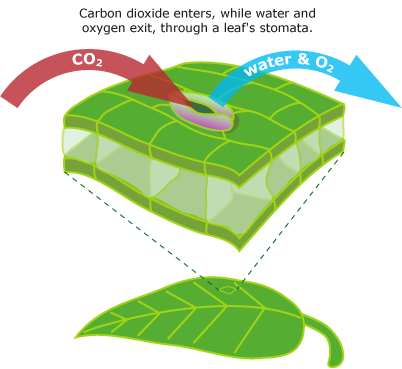
\includegraphics[width=2.25in]{stomata.png}% was O(1.5in)
        \caption{from evolution.berkeley.edu}
      \end{figure}
    \end{column}
  \end{columns}
\end{frame}


\begin{frame}{The question is, which effect dominates with an increase in VPD: plant response (decrease in ET) or atmospheric demand (increase in ET)?}
  \begin{itemize}
  \item Prior expectation:
    \begin{itemize}
    \item Should be a function of plant type: plants that are evolved to conserve water will tend to reduce ET with increases in VPD.
    \item But the environment still matters: if the atmosphere dries enough, plant water conservation strategies will reach their limit and atmospheric demand will drive increases in ET with increases in VPD.
    \end{itemize}
  \end{itemize}
\end{frame}

\section{Method}
\begin{frame}{Develop a theory to quantify VPD effects}
  \begin{itemize}
  \item The goal is to simply the problem (increase transparency) while still capturing the leading order behavior the system.
    \begin{itemize}
    \item While simplifying the system aids intrinsic understanding, simplifying assumptions sacrifice physical realism.
    \end{itemize}
  \item Because we run the risk of over-simplification, we will use FLUXNET2015 data to test how well our theory matches the data. 
  \end{itemize}
\end{frame}

\begin{frame}{Simple theory - start with Penman-Monteith}
  We can use Penman-Monteith (PM) to estimate ET:
    \[ET = \frac{\Delta R + g_a \rho_a c_p \, VPD}{\Delta + \gamma(1 + \frac{g_a}{\textcolor{magenta}{\boldsymbol{g_s}}})},\]
  \begin{overprint}
    \onslide<2>
    \textbf{Problem}: \Large $\textcolor{magenta}{\boldsymbol{g_s}}$ \normalsize (stomatal conductance) is a function of photosynthesis, which is a function of ET itself.  So ET in Penman-Monteith is really an implicit function of itself and we cannot take derivatives!<2>
  \end{overprint}
\end{frame}

\begin{frame}{Use physically reasonable assumptions remove implicit dependence}
Apply a constant uWUE assumption (conserved within plant type; see \cite{Zhou_2016}):
\[uWUE = \frac{GPP \cdot \sqrt{VPD}}{ET},\]
To derive a new form of Penman-Monteith without implicit ET dependence:
  \[  ET = \frac{\Delta R + \frac{g_a\; P}{T} \left( \frac{ c_p \, VPD}{R_{air}} -  \frac{\gamma c_s \sqrt{VPD} }{ R* \; 1.6 \text{ uWUE } (1 + \frac{g_1}{\sqrt{VPD}})} \right)}{ \Delta + \gamma}\]
\end{frame}

\begin{frame}{Now just take $\frac{\partial \; ET}{\partial \; VPD}$}
  With our new form of Penman-Monteith we can now take derivatives, giving:
  \[\frac{\partial \;  ET}{\partial \, VPD} = \frac{2 g_a \; P}{T(\Delta + \gamma)}   \left(\frac{ c_p}{R_{air}} - \frac{\gamma c_s }{1.6 \; R*\; \text{ uWUE }} \left( \frac{2 g_1 + \sqrt{VPD}}{2 (g_1 + \sqrt{VPD})^2}\right) \right)\]
  In the interest of time, we will just focus in the ``sign'' term:
  \[\sign \left[\frac{\partial \;  ET}{\partial \, VPD}\right] = \sign \left[  \left(\frac{ c_p}{R_{air}} - \frac{\gamma c_s }{1.6 \; R*\; \text{ uWUE }} \left( \frac{2 g_1 + \sqrt{VPD}}{2 (g_1 + \sqrt{VPD})^2}\right) \right) \right] \]

\end{frame}

\section{Results - theory}
\begin{frame}{Consequences of theory - ``sign'' term}
  \[\frac{\partial \, ET}{\partial \, VPD} = \text{scaling} \cdot \left(\frac{\textcolor{magenta}{\boldsymbol{ c_p}}}{R_{air}} - \frac{\gamma c_s }{1.6 \; \textcolor{magenta}{\boldsymbol{R*}}\; \text{ uWUE }} \left( \frac{2 g_1 + \sqrt{VPD}}{2 (g_1 + \sqrt{VPD})^2}\right) \right)\]
  \begin{itemize}
  \item $\textcolor{magenta}{\boldsymbol{c_p}}$ and $\textcolor{magenta}{\boldsymbol{R*}}$ are constants
  \end{itemize}
\end{frame}

\begin{frame}{Consequences of theory - ``sign'' term}
  \[\frac{\partial \, ET}{\partial \, VPD} = \text{scaling} \cdot \left(\frac{ c_p}{\textcolor{magenta}{\boldsymbol{R_{air}}}} - \frac{\textcolor{magenta}{\boldsymbol{\gamma}} \textcolor{magenta}{\boldsymbol{c_s}} }{1.6 \; R*\; \text{ uWUE }} \left( \frac{2 g_1 + \sqrt{VPD}}{2 (g_1 + \sqrt{VPD})^2}\right) \right)\]
  \begin{itemize}
  \item $c_p$ and $R*$ are constants
  \item $\textcolor{magenta}{\boldsymbol{R_{air}}}$, $\textcolor{magenta}{\boldsymbol{\gamma}}$, and $\textcolor{magenta}{\boldsymbol{c_s}}$ are approximately constant (relative to $\sqrt{VPD}$)
  \end{itemize}
\end{frame}

\begin{frame}{Consequences of theory - ``sign'' term}
  \[\frac{\partial \, ET}{\partial \, VPD} = \text{scaling} \cdot \left(\frac{ c_p}{R_{air}} - \frac{\gamma c_s }{1.6 \; R*\; \text{ \textcolor{magenta}{\textbf{uWUE }}}} \left( \frac{2 \textcolor{magenta}{\boldsymbol{g1}} + \sqrt{VPD}}{2 (\textcolor{magenta}{\boldsymbol{g1}} + \sqrt{VPD})^2}\right) \right)\]
  \begin{itemize}
  \item $c_p$ and $R*$ are constants
  \item $R_{air}$, $\gamma$, and $c_s$ are approximately constant (relative to $\sqrt{VPD}$)
  \item \textcolor{magenta}{\textbf{uWUE}} and $\textcolor{magenta}{\boldsymbol{g1}}$ are constants within plant type (e.g. grass, crops, deciduous broadleaf forest, evergreen needleleaf forest, shrub)
  \end{itemize}
  So within each plant type, whether the atmospheric demand (ET increasing with VPD) or plant response (ET decreasing with VPD) dominates is essentially just a function of VPD!
\end{frame}

\begin{frame}{Consequences of theory - ``sign'' term}
  \[\frac{\partial \, ET}{\partial \, VPD} = \text{scaling} \cdot \left(\frac{ c_p}{R_{air}} - \frac{\gamma c_s }{1.6 \; R*\; \text{ uWUE }} \left( \frac{2 g1 + \sqrt{VPD}}{2 (g1 + \sqrt{VPD})^2}\right) \right)\]
  \begin{itemize}
  \item $c_p$ and $R*$ are constants
  \item $R_{air}$, $\gamma$, and $c_s$ are approximately constant (relative to $\sqrt{VPD}$)
  \item uWUE and $g1$ are constants within plant type (e.g. grass, crops, deciduous broadleaf forest, evergreen needleleaf forest, shrub)
  \end{itemize}
  So \textbf{within each plant type}, whether the atmospheric demand (ET increasing with VPD) or plant response (ET decreasing with VPD) dominates is approximately \textbf{just a function of VPD}!
\end{frame}


\begin{frame}{``Sign'' term as a function of VPD and PFT}
  \begin{figure}
      \begin{tikzpicture}
    \node[anchor=south west,inner sep=0] (image) at (0,0) {\adjincludegraphics[width=3.3in, trim={0 {0.51\height} 0 0}, clip]{fig05.pdf}};
        \begin{scope}[x={(image.south east)},y={(image.north west)}]
        %% next four lines will help you to locate the point needed by forming a grid. comment these four lines in the final picture.↓
       % \draw[help lines,xstep=.1,ystep=.1] (0,0) grid (1,1);
       % \draw[help lines,xstep=.05,ystep=.05] (0,0) grid (1,1);
       % \foreach \x in {0,1,...,9} { \node [anchor=north] at (\x/10,0) {0.\x}; }
       % \foreach \y in {0,1,...,9} { \node [anchor=east] at (0,\y/10) {0.\y};}
       %% upto here
        \draw[-latex, line width=2pt] (0.83,0.725) --++(0.0in,0.3in)node[anchor=south] {ET Increasing};
        \draw[-latex, line width=2pt] (0.83,0.725) --++(0.0in,-0.3in)node[anchor=north] {ET Decreasing};

        % \draw[dashed,-latex, line width=5pt] (0.8,0.75) --++(0.0in,+0.5in)node[anchor=north] {ET Decreasing};
    \end{scope}
    % \node[align=center,red,font={\large}] at (image.southwest) {ET decreasing};
  \end{tikzpicture}
  \end{figure}
\end{frame}


\begin{frame}{``Sign'' term as a function of VPD and PFT}
  \begin{figure}
      \begin{tikzpicture}
    \node[anchor=south west,inner sep=0] (image) at (0,0) {\adjincludegraphics[width=3.3in, trim={0 {0.51\height} 0 0}, clip]{fig05_pet.pdf}};
        \begin{scope}[x={(image.south east)},y={(image.north west)}]
        %% next four lines will help you to locate the point needed by forming a grid. comment these four lines in the final picture.↓
       % \draw[help lines,xstep=.1,ystep=.1] (0,0) grid (1,1);
       % \draw[help lines,xstep=.05,ystep=.05] (0,0) grid (1,1);
       % \foreach \x in {0,1,...,9} { \node [anchor=north] at (\x/10,0) {0.\x}; }
       % \foreach \y in {0,1,...,9} { \node [anchor=east] at (0,\y/10) {0.\y};}
       %% upto here
        % \draw[-latex, line width=2pt] (0.83,0.725) --++(0.0in,0.3in)node[anchor=south] {ET Increasing};
        % \draw[-latex, line width=2pt] (0.83,0.725) --++(0.0in,-0.3in)node[anchor=north] {ET Decreasing};
        % \draw[dashed,-latex, line width=5pt] (0.8,0.75) --++(0.0in,+0.5in)node[anchor=north] {ET Decreasing};
    \end{scope}
    % \node[align=center,red,font={\large}] at (image.southwest) {ET decreasing};
  \end{tikzpicture}
\end{figure}
\begin{textblock*}{0.25\textwidth}(0.02\textwidth,0.3\textheight)
  \textcolor{magenta}{Dashed line} gives response for potential evapotranspiration (PET).\\
\medskip
  Plants are crucial for land response!
\end{textblock*}
\end{frame}


\section{Test Theory}
\begin{frame}{The theory seems nice, but we need to test with data!}
  \begin{itemize}
  \item Introduce a free uncertainty parameter \Large $\textcolor{magenta}{\boldsymbol{\sigma}}$ \normalsize to Penman Monteith:
    \[ET = \frac{\Delta R + \frac{g_a\; P}{T} \left( \frac{ c_p VPD}{R_{air}} -  \frac{\gamma c_s \sqrt{VPD} }{ R* \; 1.6\; \textcolor{magenta}{\boldsymbol{\mathlarger{\sigma}}} \; \text{ uWUE } (1 + \frac{g_1}{\sqrt{VPD}})} \right) }{ \Delta + \gamma}\]
  \item At each observation from FLUXNET (56 sites) calculate a unique \Large $\textcolor{magenta}{\boldsymbol{\sigma}}$ \normalsize:
    \[\textcolor{magenta}{\boldsymbol{\mathlarger{\sigma}}}(t, \text{site}) = f(ET_{obs})\]

    \item Then propagate uncertainty forward by including \Large $\textcolor{magenta}{\boldsymbol{\sigma}}$ \normalsize in the derivative:
    \end{itemize}
      \[\frac{\partial \;  ET}{\partial \; VPD} = \text{scaling} \cdot \left(\frac{ c_p}{R_{air}} -  \frac{\gamma c_s }{1.6 \; R*\; \textcolor{magenta}{\boldsymbol{\mathlarger{\sigma}}} \; \text{ uWUE }} \left( \frac{2 g_1 + \sqrt{VPD}}{2 (g_1 + \sqrt{VPD})^2}\right) \right)\]
\end{frame}
  
\begin{frame}{Test theory with FLUXNET data - the good}
  \begin{columns}
    \begin{column}{0.33\textwidth}
      \includegraphics[width=1.2\textwidth]{DBF_box.pdf}
    \end{column}
    \begin{column}{0.33\textwidth}
    \end{column}
    \begin{column}{0.33\textwidth}
    \end{column}
  \end{columns}
\end{frame}

\begin{frame}{Test theory with FLUXNET data - the good}
  \begin{columns}
    \begin{column}{0.33\textwidth}
      \includegraphics[width=1.2\textwidth]{DBF_box.pdf}
    \end{column}
    \begin{column}{0.33\textwidth}
      \includegraphics[width=1.2\textwidth]{ENF_box.pdf}
    \end{column}
    \begin{column}{0.33\textwidth}
      \includegraphics[width=1.2\textwidth]{CSH_box.pdf}
    \end{column}
  \end{columns}
\end{frame}


\begin{frame}{Test theory with FLUXNET data - the bad}
    \begin{columns}
    \begin{column}{0.5\textwidth}
      \includegraphics[width=\textwidth]{GRA_box.pdf}
    \end{column}
    \begin{column}{0.5\textwidth}
      \includegraphics[width=\textwidth]{CRO_box.pdf}
    \end{column}
  \end{columns}
\end{frame}



% \begin{frame}{Summary of theory}
%   \begin{itemize}
%   \item We use \cite{Zhou_2016}'s uWUE to derive a new analytically tractable form of PM.
%   \item This new analysis suggests that the ``tipping'' point for which atmospheric demand overwhelms plant response will be almost exclusively a function of VPD.
%     \begin{itemize}
%     \item For each PFT there will be a VPD$_{crit}$ above which atmospheric demand will dominate and ET will increase with VPD.
%     \end{itemize}
%   \item Plant types evolved to conserve water (CSH) have a higher VPD$_{crit}$ than plants evolved (or bred) to use water and prioritize GPP (CRO). Trees and grasslands are somewhere between these two extremes.
%   \item Aerodynamic conductance scales the response, so plants with large surface roughness will be more likely to have a larger response as there is less resistance between the surface and the atmosphere.
%   \end{itemize}
% \end{frame}


\section{Conclusions}
% \begin{frame}{Summary}
%   \begin{itemize}
%   \item Theory finds that the ``tipping'' point for which atmospheric demand overwhelms plant response will be almost exclusively a function of VPD.  Plant types evolved to conserve water (CSH) have a higher VPD$_{crit}$ (and more negative ET response) than plants evolved (or bred) to use water and prioritize GPP (CRO).
%   \item On average, ecosystem response to VPD follows roughly what we might expect: CRO (prioritize GPP) has positive ET response to VPD, while all others have a negative response. Ordering by increasing magnitude of negative response gives: DBF, GRA, ENF, CSH; which roughly correspond to expectations for increasing water conservation as a function of PFT.
%   \item Uncertainty is high, especially for CRO and GRA. However, inclusion of uncertainty does not change the story for ENF or CSH.
%   \end{itemize}
% \end{frame}


\begin{frame}{Summary - When does VPD drive or reduce ET?}
  \begin{itemize}
  \item Theory predicts that each plant type has a \textbf{critical VPD} \textbf{below which ET will decrease} (plant response dominates), and \textbf{above which ET will increase} (atmosheric demand dominsates).
  \item For forest sites, environmental VPD approximately straddles the critical VPD.
  \item For shrubs environmental VPD never exceeds the critical VPD.
  \item Theory tested poorly with FLUXNET data for for crops and grass. 
  \item All plant types exhibited a response far below that of PET.
  \item The new uWUE-version of Penman-Monteith we derived could be used as a replacement for PET in drought indices over vegetated surfaces.
  \end{itemize}
\end{frame}

\section{References}
\begin{frame}{References}
  \AtNextBibliography{\small}
  \printbibliography
  \scriptsize
  \begin{itemize}
  \item This work used eddy covariance data acquired and shared by the FLUXNET community, including these networks: AmeriFlux, AfriFlux, AsiaFlux, CarboAfrica, CarboEuropeIP, CarboItaly, CarboMont, ChinaFlux, Fluxnet-Canada, GreenGrass, ICOS, KoFlux, LBA, NECC, OzFlux-TERN, TCOS-Siberia, and USCCC. The ERA-Interim reanalysis data are provided by ECMWF and processed by LSCE. The FLUXNET eddy covariance data processing and harmonization was carried out by the European Fluxes Database Cluster, AmeriFlux Management Project, and Fluxdata project of FLUXNET, with the support of CDIAC and ICOS Ecosystem Thematic Center, and the OzFlux, ChinaFlux and AsiaFlux offices.
    \item This material is based upon work supported by the National Science Foundation Graduate Research Fellowship under Grant No. DGE 16-44869. Any opinion, findings, and conclusions or recommendations expressed in this material are those of the authors(s) and do not necessarily reflect the views of the National Science Foundation.
    \end{itemize}
\end{frame}

\section{Extra Slides}

\begin{frame}{Extra slide - statistics}
  \begin{table}
  \label{vpd_crit}
\caption{More quantitative test of theory.}
\centering
\begin{tabular}{l c c c c c c}
  \hline
  PFT & \specialcell{Fraction of Obs.\\Theory is Correct} & Mean ($\frac{\partial \; ET}{\partial \; VPD} < 0$) & Mean ($\frac{\partial \; ET}{\partial \; VPD} > 0$)\\
  \hline
  CRO & 0.566517 & -0.209152 &  0.005856\\
  CSH & 0.931660 & -0.264746 &       NaN\\
  DBF & 0.633363 & -0.135679 &  0.042910\\
  ENF & 0.633138 & -0.150665 &  0.029281\\
  GRA & 0.442306 & -0.042158 & -0.042480\\
  \hline
\end{tabular}
\end{table}
\end{frame}

\begin{frame}{Extra slide - is theory VPD$_{crit}$ optimum?}
  \includegraphics[width=0.7\textwidth]{for_agu.pdf}
\end{frame}

\begin{frame}{Test theory with FLUXNET data - CSH}
  \includegraphics[width=3.5in]{csh_eee.png}
\end{frame}

\begin{frame}{Test theory with FLUXNET data - ENF}
  \includegraphics[width=3.5in]{enf_eee.png}
\end{frame}

  
\begin{frame}{Test theory with FLUXNET data - DBF}
  \includegraphics[width=3.5in]{dbf_eee.png}
\end{frame}

\begin{frame}{Test theory with FLUXNET data - CRO}
  \includegraphics[width=3.5in]{cro_eee.png}
\end{frame}

\begin{frame}{Test theory with FLUXNET data - GRA}
  \includegraphics[width=3.5in]{gra_eee.png}
\end{frame}


% \begin{frame}{Summary statistics - extra sl}
%      \begin{table}
%        \caption{Statistics of $\frac{\partial \; ET}{\partial \, VPD}$ as a function of PFT.}
%        \centering
%        \begin{tabular}{l c c}
%          \hline
%          PFT & $\overline{\frac{\partial \; ET}{\partial \; VPD}}$ & fraction $\frac{\partial \; ET}{\partial \; VPD} < 0.$ \\
%          \hline
%          CRO & 0.000853  & 0.473311\\
%          CSH & -0.108234 & 0.931660\\
%          DBF & -0.012727 & 0.461674\\
%          ENF & -0.034087 & 0.534425\\
%          GRA & -0.019637 & 0.631735\\
%          \hline
%          \multicolumn{2}{l}{}  
%        \end{tabular}
%      \end{table}
%    \end{frame}
     




% \begin{table}
% \centering
% \begin{tabular}{l|r}
% Item & Quantity \\\hline
% Widgets & 42 \\
% Gadgets & 13
% \end{tabular}
% \caption{\label{tab:widgets}An example table.}
% \end{table}

\end{document}
